\documentclass[a4paper, twocolumn]{article}

% you can switch between these two (and more) styles by commenting one out (use percentage)
\usepackage[backend=biber]{biblatex}
%\usepackage[backend=biber, style=authoryear-icomp]{biblatex}
\addbibresource{./refs.bib}
\usepackage{graphicx}
\usepackage{listings}
\usepackage{color}
\usepackage{titlesec}
\usepackage{titling}
\usepackage{geometry}
 \geometry{
 a4paper,
 total={170mm,257mm},
 left=20mm,
 right=20mm,
 top=20mm,
 bottom=30mm,
 }

\titlespacing\section{0pt}{10pt plus 4pt minus 2pt}{0pt plus 2pt minus 2pt}
\definecolor{lightgray}{gray}{0.9}

% code listing: https://tex.stackexchange.com/questions/19004/how-to-format-an-inline-source-code
\lstset{
    showstringspaces=false,
    basicstyle=\ttfamily,
    keywordstyle={blue},
    commentstyle=\color[gray]{0.6}
    stringstyle=\color[RGB]{255, 150, 75}
}
\newcommand{\inlinecode}[2]{\colorbox{lightgray}{\lstinline[language=#1]$#2$}}

\setlength{\droptitle}{-2em}

\author{Michael Sungsoo Fuglø, Michael Kwabena Berko, Julius Stenbæk Christoffersen}
\title{Enhancing Seafood Supply Chain Management through Convolutional Neural Networks: A Case Study of Fish Classification Using Visual Features}
\date{April 2023}

\begin{document}

\twocolumn[
    \begin{@twocolumnfalse}
        \maketitle
        \begin{abstract}
            This paper investigates the use of convolutional neural networks to accurately classify nine different types of fish based on their visual features. The aim is to help seafood vendors and regulators quickly identify and manage their seafood supply chain. An image dataset consisting of fish taken from cutting boards at a fish market in Izmir, Turkey was used to train a machine learning model. The model achieved an accuracy of 96\% on the test set. A pre-trained MobileNetV2 model was also used and achieved an accuracy of 99.9\% on the test set. This suggests that transfer learning using a pre-trained model is an effective strategy for this use case.  
        \end{abstract}
    \end{@twocolumnfalse}
    \vspace{1cm}
]

\section{Problem\label{sec:Problem}}

Fish markets play a vital role in the seafood industry by providing fresh seafood to consumers. Accurate identification of fish species is important in this industry for ensuring that consumers and retailers can avoid food forgery by fish providers. However, identifying fish species can be challenging, especially when dealing with a large number of different species. \cite{10.1371/journal.pone.0012620}

This led us to the following research question:
Given an image dataset of 9 different types of fish taken from cutting boards at a fish market in Izmir, Turkey, can we accurately classify each fish based on its visual features?

\section{Objective\label{sec:Objective}}


The objective of this problem is to build a machine-learning model that can accurately classify each fish species based on its visual features. This model could be used to help seafood vendors and regulators to quickly identify and manage the seafood supply chain, ensuring that the seafood is labeled correctly and is safe for consumption. 

Additionally, the model could be used by customers who are looking for specific types of fish to help them make informed purchasing decisions.


\section{Hypothesis\label{sec:Hypothesis}}

There is a statistically significant difference in the visual features of each type of fish (e.g. gilt head bream, red sea bream, sea bass, etc.), such that each type can be accurately identified based on its unique visual characteristics.

Giving us the following null hypothesis:
There is no statistically significant difference in the visual features of each type of fish (e.g. gilt head bream, red sea bream, sea bass, etc.), such that accurate identification of each type based on visual characteristics is not possible.

\section{Dataset\label{sec:Dataset}}
The dataset consists of images of 9 different types of fish that are sold in a fish market in Izmir. The images are taken from cutting boards at the fish market and each fish is labeled with its corresponding species. The fish images appear in different rotational angles, but are always displayed on identical blue cutting boards. \cite{ulucan2020large}

\section{Method}\label{sec: Method}
 The dataset was divided into training, validation, and test sets with a ratio of 75:10:15 respectively. We also ensured that there was no overlap between the images in these three sets.
 
To ensure that the CNN model could process the dataset effectively, we rescaled all the images to a size of 224x224 pixels, which is a commonly used size for CNN models.
\cite{Talebi_2021_ICCV}

The CNN model requires the target variable (fish species in this case) to be in a numerical format. To convert the categorical target variable into a numerical format, we used 1-hot encoding. In our case, we had 9 different fish species, so we created a binary vector of size 9 for each image, where the index of the fish species was marked as 1, and the rest were marked as 0. This ensured that the target variable was in a numerical format that could be processed by the CNN model.

\section{Analysis}\label{sec: Analysis}
We designed a CNN architecture consisting of four convolutional layers, and two dropout layers to combat overfitting of the model. We used a ReLU activation function after each convolutional layer. Finally, a softmax activation function was used in the output layer to classify the images into one of the 9 fish species.

\subsection{Training and Evaluation}\label{sec: Training and Evaluation}
The CNN model was trained on the augmented dataset using the categorical cross-entropy loss function and the Adam optimizer. We trained the model for 30 epochs with a batch size of 32. We used the validation set to tune the hyperparameters of the model such as the learning rate and the number of filters in the convolutional layers. We evaluated the model on the test set and reported the accuracy and confusion matrix to measure the performance of the model.

\begin{figure}[h]
\centering
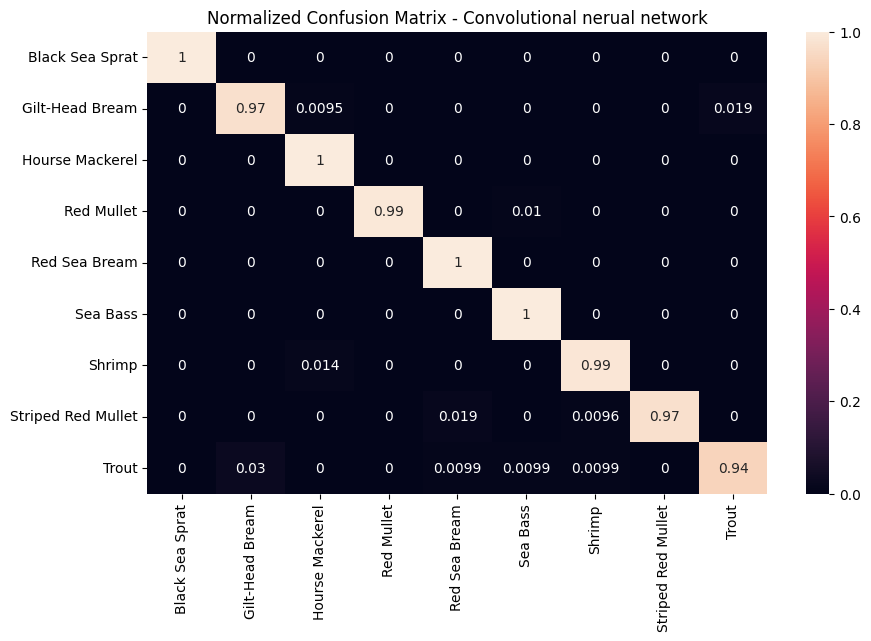
\includegraphics[width=0.5\textwidth]{figures/confusion_matrix_CCN.png}
\caption{Normalized Confusion Matrix for Our CNN.}
\label{fig:example}
\end{figure}

\subsection{Using a Pre-Trained Model}\label{sec: Using a Pre-Trained Model}
After creating our own CNN model, we also used a pre-trained model, MobileNetV2, which is a popular CNN architecture that has been pre-trained on a large dataset of images.
\cite{9422058}

We froze the layers in MobileNetV2 up to the last convolutional block and trained the last layer on our fish dataset. We used the same data augmentation techniques and split the dataset into the same training, validation, and test sets as before. We trained the MobileNetV2 model for 10 epochs with a batch size of 32. Again we used the categorical cross-entropy loss function and the Adam optimizer. We evaluated the model on the test set and reported the accuracy and confusion matrix to measure the performance of the model.

\begin{figure}[h]
\centering
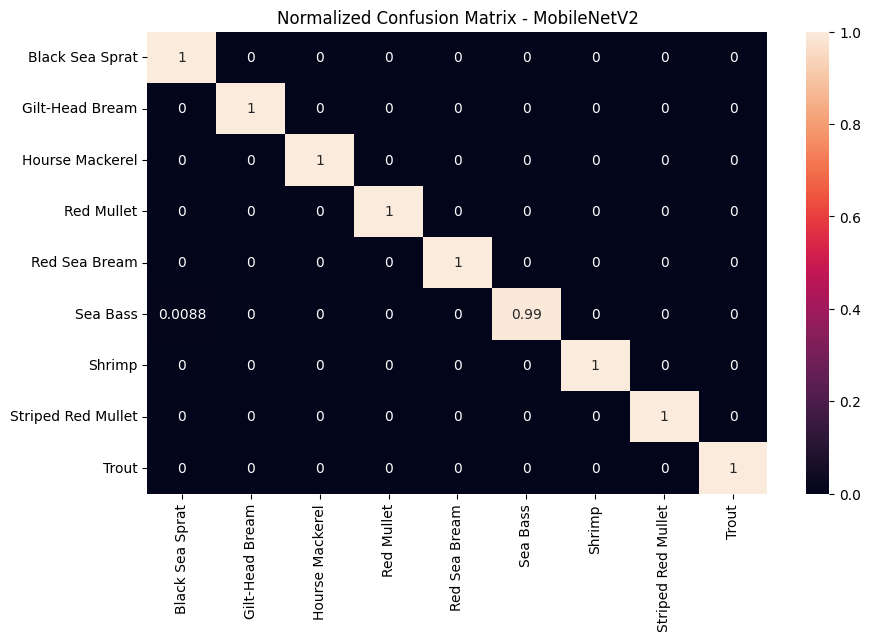
\includegraphics[width=0.5\textwidth]{figures/confusion_matrix_pretrained.png}
\caption{Normalized Confusion Matrix for Pre-Trained Model.}
\label{fig:example}
\end{figure}

\section{Findings}\label{sec: Findings}
Our own CNN model achieved an accuracy of 96\% on the test set. The confusion matrix showed that the model was able to predict the 9 types of fish in images with high accuracy. The highest accuracy was achieved by the black sea sprat, the house mackerel, the red sea bream and the sea bass of 100\%, while the lowest accuracy was for the trout species with 93\% accuracy.

The pre-trained MobileNetV2 model achieved an accuracy of 99.9\% on the test set, which was higher than the accuracy achieved by our own CNN model. The only fish species without a 100\% accuracy on the test set was the sea bass species with 99.9\% accuracy.


\section{Conclusion}\label{sec: Conclusion}
In summary, our study used Convolutional Neural Networks to accurately predict 9 types of fish in images. We created our own CNN model and used a pre-trained model, MobileNetV2, to predict the fish species. The pre-trained model achieved higher accuracy than our own CNN model, suggesting that transfer learning using pre-trained models is a useful technique.

Having been trained on a limited dataset of 9 different species of fish, the model won't be able to solve seafood supply chain issues by itself. However, our findings carry results of significant value suggesting that further development of a computer vision model using a CNN architecture would help seafood supply chain vendors and regulators accurately identify different species of fish.

\printbibliography
\end{document}
